% Pixel Function Manager

The pixel Level 1 function manager (L1FM or FM) acts as an interface 
between the global run control (the Level 0 function manager, RCMS 
for Run Control and Monitoring System) and the pixel online 
software.  The FM is a java application.  It implements the state 
machine of CMS~\cite{statemachine}.  It responds to requests from 
RCMS to change states in the state diagram that describes the state 
of the DAQ system.  This state diagram is shown in 
Fig.~\ref{fig:l1fm}.  The function manager interacts with the 
PixelSupervisor to carry out the different tasks needed in state 
transitions of the run control.  The pixel FM is a relatively thin 
layer that basically just passes the state changes on to the 
PixelSupervisor.

\begin{figure}
\begin{center}
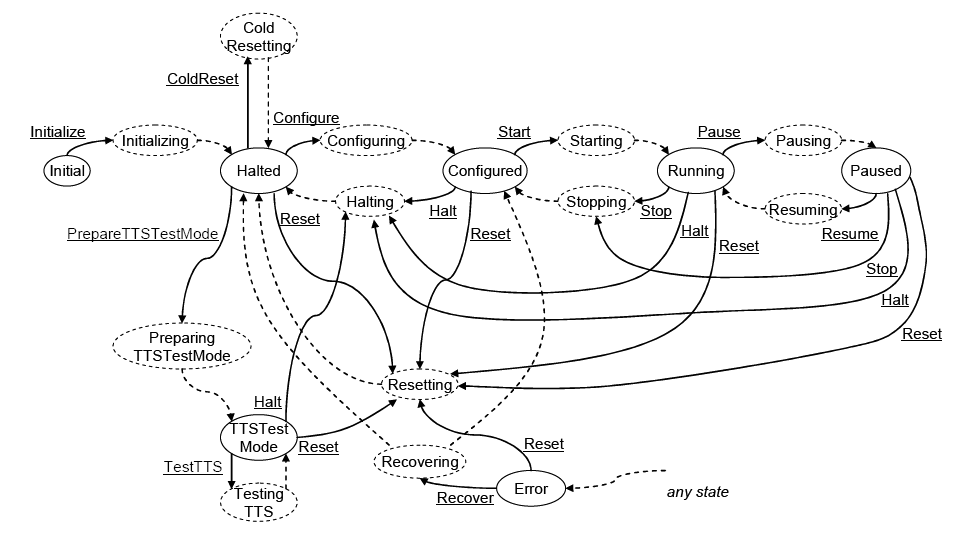
\includegraphics[width=0.99\textwidth]{l1fm_states.png}
\end{center}
\caption{The CMS finite state machine definition. Figure taken from Ref.~\cite{statemachine}.}
\label{fig:l1fm}
\end{figure}

\subsection{FSM Implementation Status}
The CMS run control finite state machine (FSM) is shown in
Fig.~\ref{fig:l1fm}. This model is implemented in the the pixel
function manager, and also in the PixelSupervisor. The other
Supervisors implement portions of this model as required. At the
moment, the FSM depicted in the figure is completely implemented in
the PixelSupervisor, with the exception of the ``Reset'' transition
and its accompanying ``Resetting'' state. The PixelSupervisor does
include transitions from any state into the ''Error'' state, and then
allows a ``Recover'' transition that returns the FSM to the ``Halted''
state.

\subsection{Control of the L1FM}

During global running, the L1FM is driven by the L0FM, which is
operated by central DAQ. The pixel user should not intervene via the
L1FM GUI, except to check its status.

During local running, the L1FM must be created via its GUI. State
transitions of the FSM can then be driven via the L1FM GUI. In
general, we drive the ``Initialize'' state transition via the GUI,
then drive subsequent state transitions directly from the
PixelSupervisor. However, in principle all transitions can be
initiated from the L1FM GUI.\footnote{In practice, this is only useful for simple tests of the L1FM to PixelSupervisor communication.}

\subsection{Outline of L1FM implementation}

The L1FM is created using the Create button in RCMS. This calls the
method of {\tt PixelFunctionManager.java} called {\tt
createAction()}.

After creation, transitions of the FM FSM are handled
by methods in {\tt PixelEventHandler.java}. Which method is triggered
depends on the transition, as defined by a table near the top of this
class. The names are fairly logical (for example, ``Initialize''
corresponds to the {\tt initAction} method and ``Configure''
corresponds to the {\tt configureAction} method). Inside each {\tt
fooAction} method are two blocks: one to handle objects of type {\tt
StateEnteredEvent} and one to handle objects of type {\tt
StateNotification}. 

When an FSM transition ``foo'' is initiated by the L0FM or L1FM GUI,
we enter the {\tt StateEnteredEvent} block of {\tt fooAction}. This
block then contains the code to send a message to PixelSupervisor,
telling it to proceed with transition ``foo''. The L1FM then does
nothing while PixelSupervisor coordinates the necessary activities in
POS. When the transition is completed by the PixelSupervisor, it
passes a message back to the L1FM.\footnote{This is implemented in
PixelSupervisor using the {\tt stateChanged} method of the {\tt
rcmsStateNotifier\_} object.} This message triggers entry into the {\tt
StateNotification} block of {\tt fooAction}. If PixelSupervisor
reports that the transition was successful, this block moves the L1FM
FSM into the state ``foo''. If PixelSupervisor reports an error, this
block moves the L1FM FSM into state ``Error''. In this way, the L0FM
(central DAQ) learns whether the transition was successful.

